\section{Үр дүн}
\subsection{Аймаг сумдын мэдээлэл авдаг форм}

\begin{figure}
	\centering
	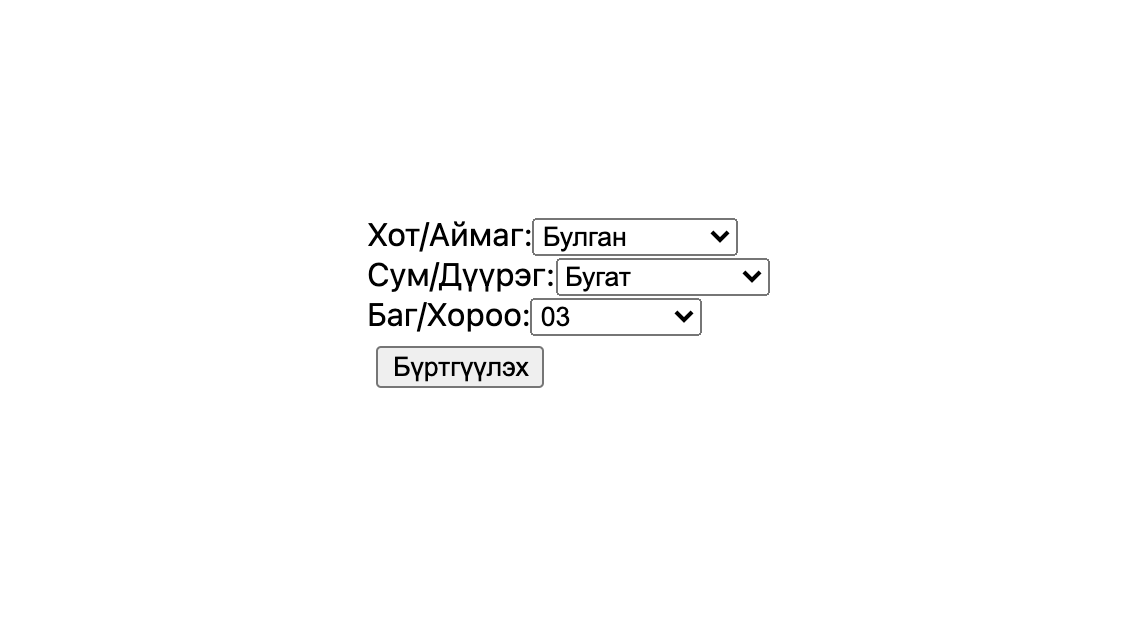
\includegraphics[width=15cm]{images/form-v1.png}
	\caption{Формын эхний хувилбар}
	\label{fig:form-v1}
\end{figure}

\begin{figure}
	\centering
	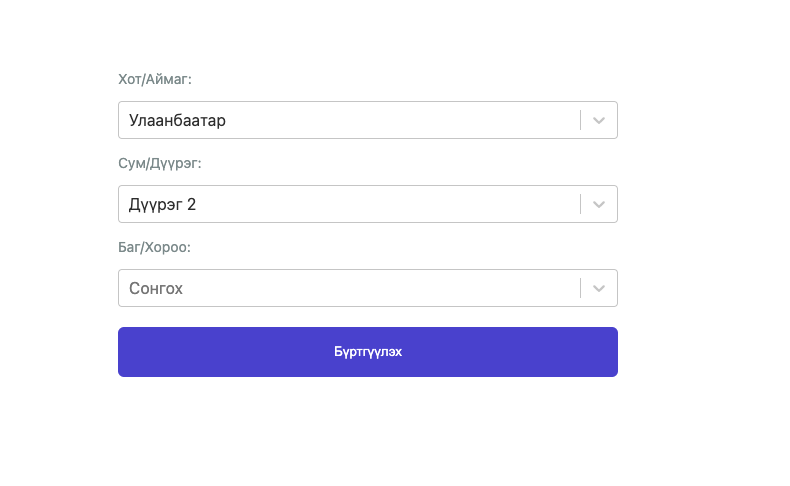
\includegraphics[width=15cm]{images/form.png}
	\caption{Material ui болон React Select ашигласан байдал}
	\label{fig:form-v2}
\end{figure}
\pagebreak

\subsection{Toast компонент}

\begin{figure}
	\centering
	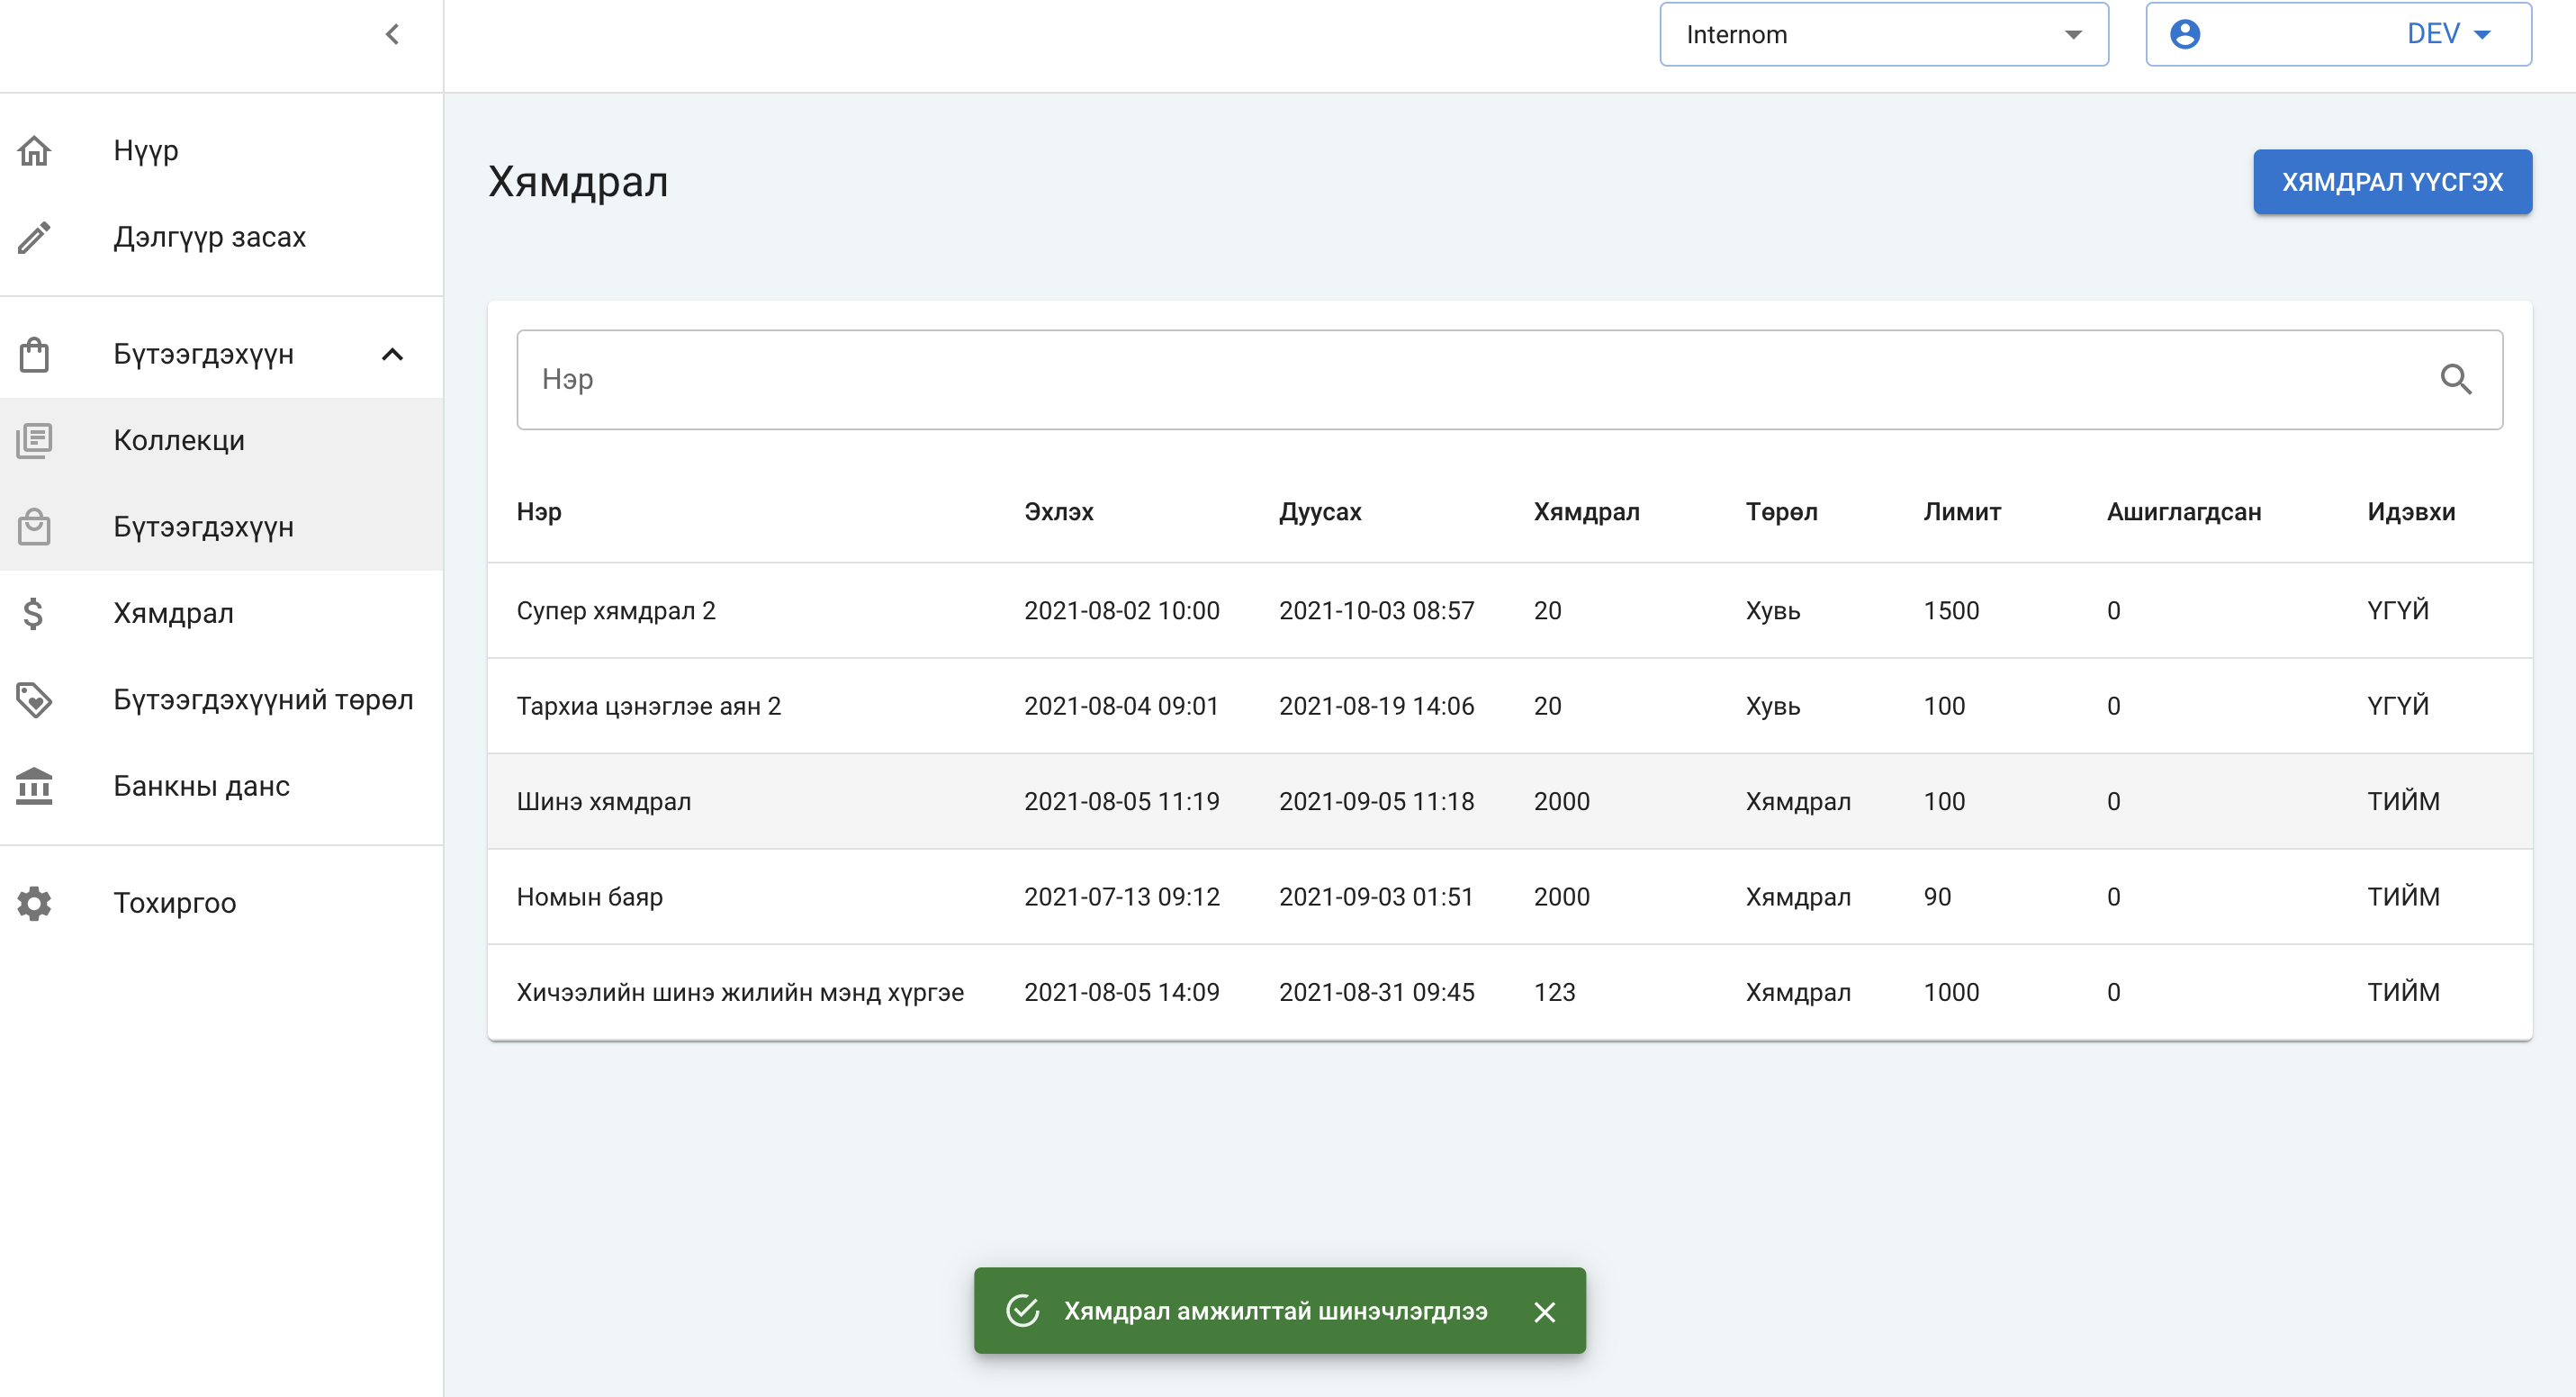
\includegraphics[width=15cm]{images/toast-success.png}
	\caption{Хүсэлт амжилттай болсон үед харагдах Toast}
	\label{fig:toast-v1}
\end{figure}

\begin{figure}
	\centering
	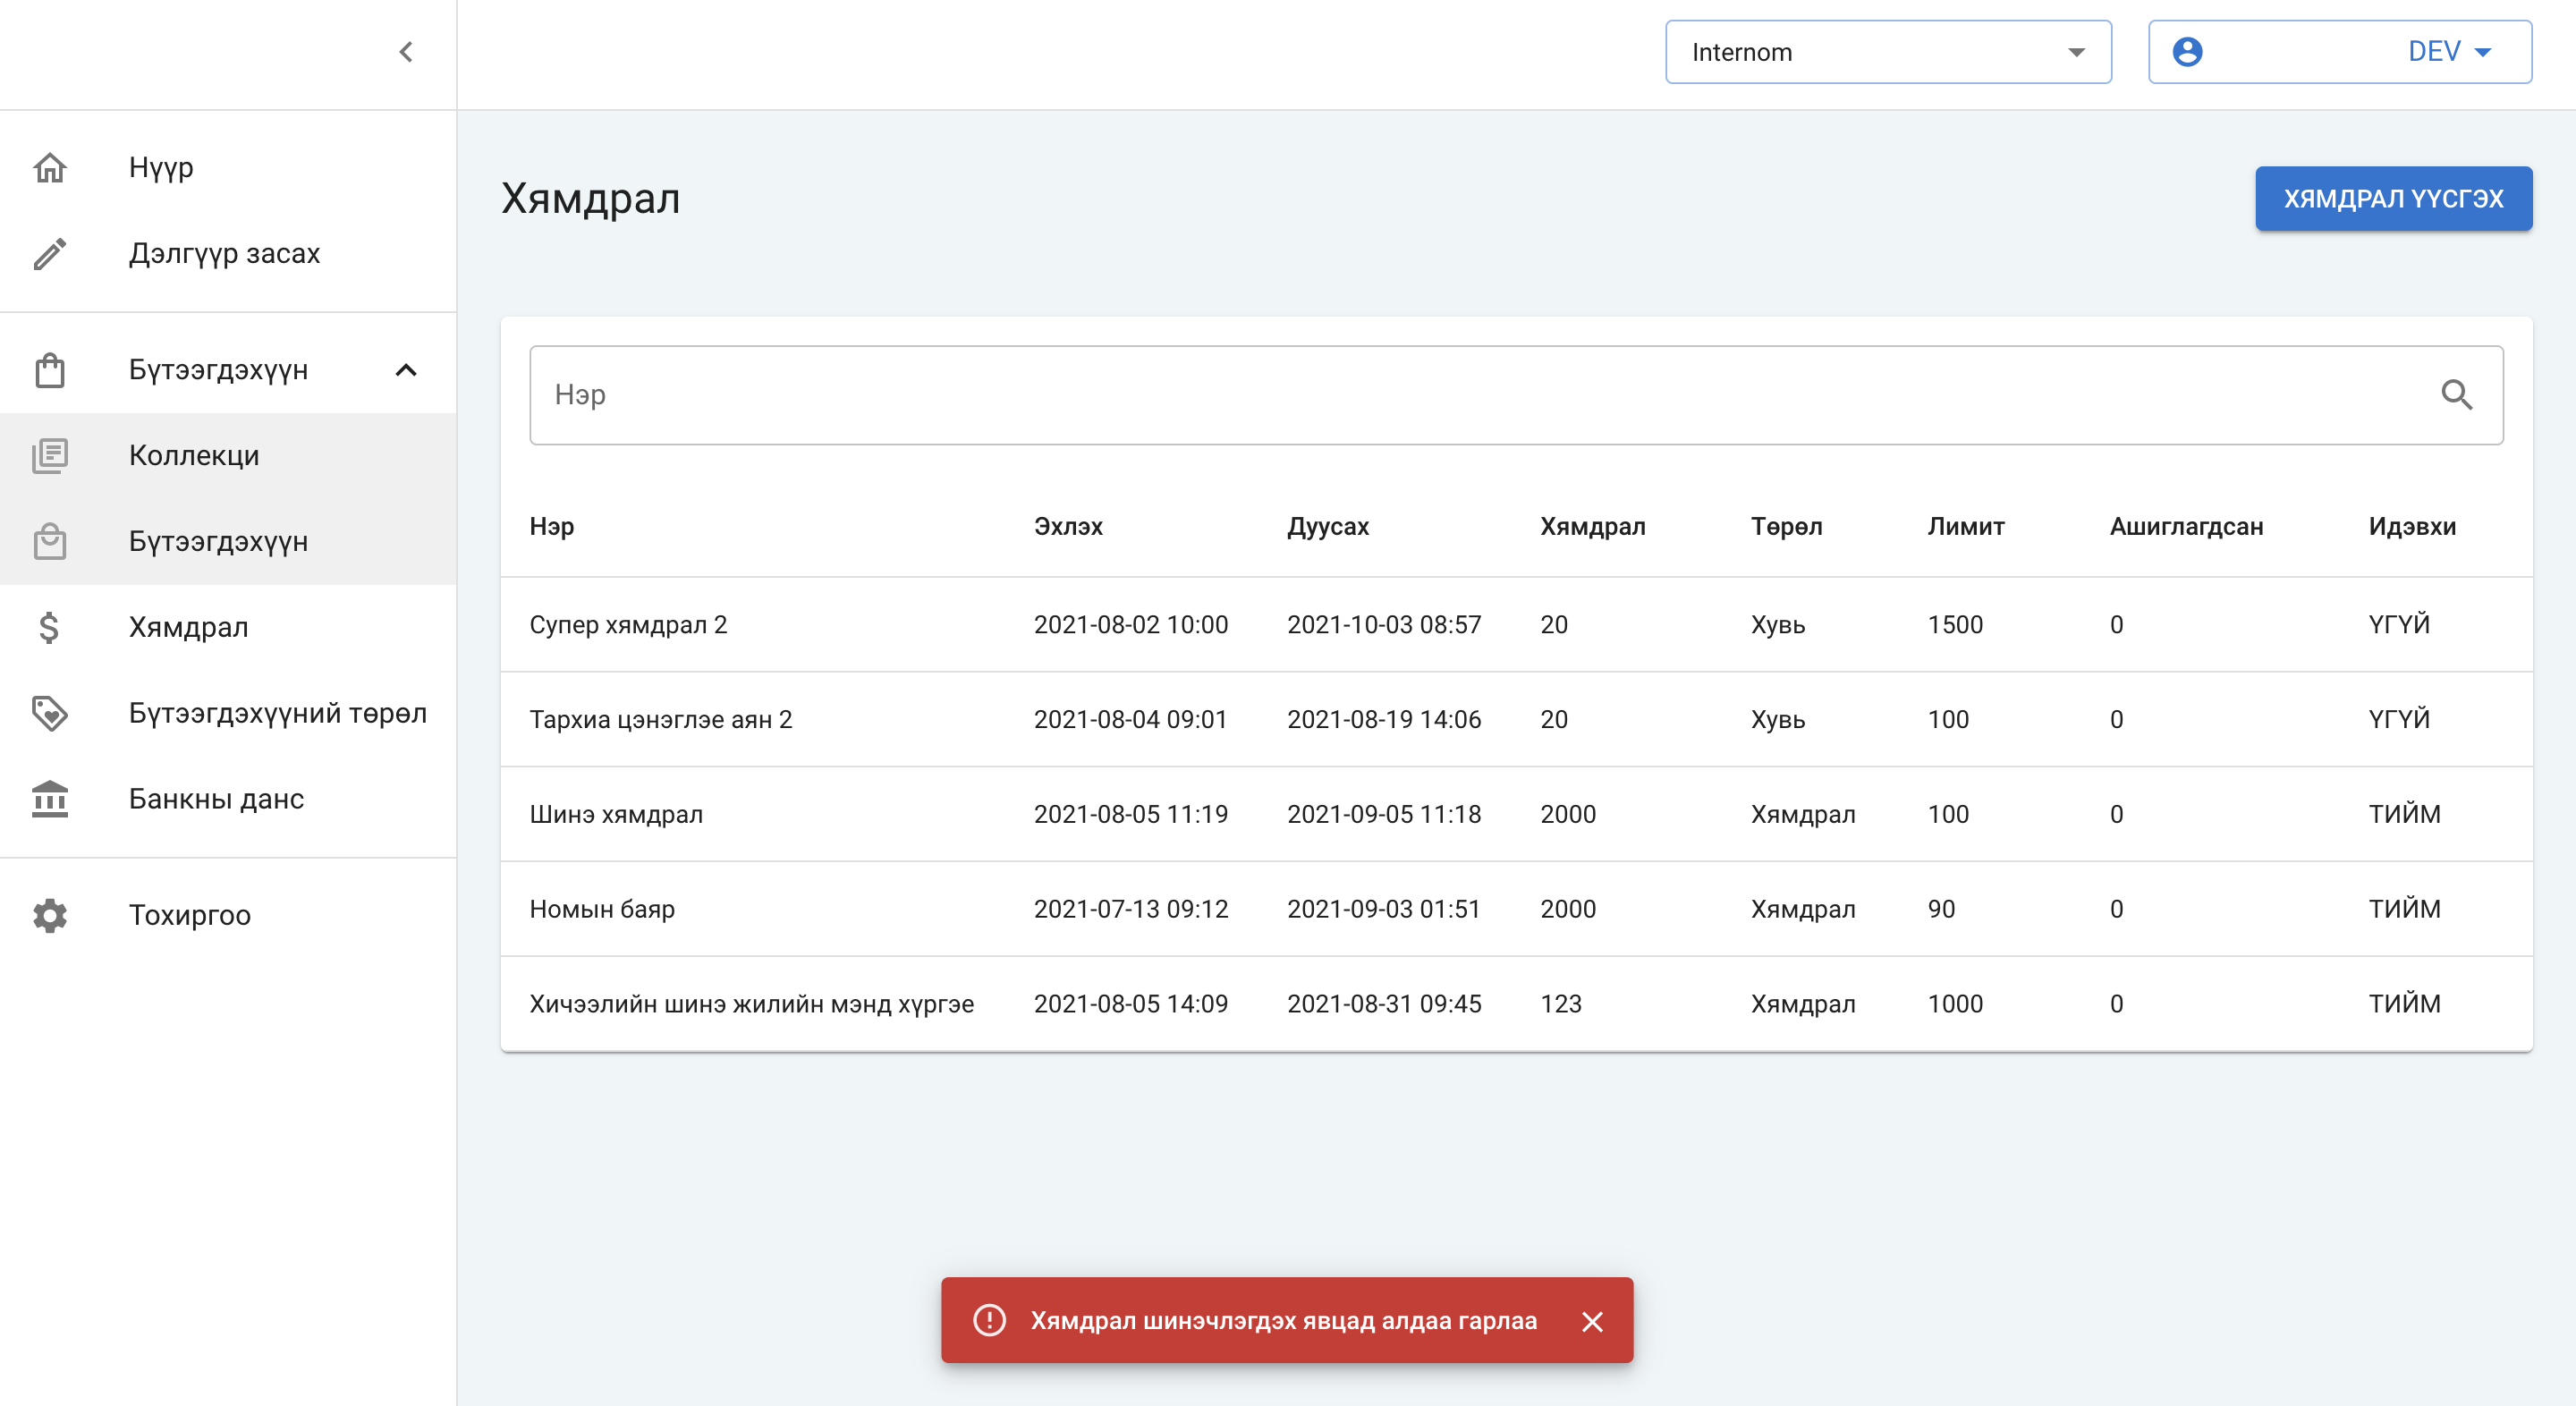
\includegraphics[width=15cm]{images/toast-failed.png}
	\caption{Хүсэлт амжилтгүй болсон үед харагдах Toast}
	\label{fig:toast-v2}
\end{figure}

\pagebreak
\section{Үр дүнгийн тайлан}
Миний бие Хуур Мюзик Групп ХХК-д 21 хоногийн хугацаатай мэргэжлийн дадлагыг амжилттай гүйцэтгэж дуусгалаа. Уг хугацаанд хичээлийн хүрээнд үзсэн онолын ойлголтуудыг практик дээр туршиж, хэрэгжүүлсэн ба хөгжүүлэлт голчилсон технологийн компанийн ерөнхий үйл ажиллагаа, баг хооронд зохицон ажиллах чадвар, хөгжүүлэлтийн шинэ арга барилуудыг амжилттай эзэмшсэн гэж дүгнэж байна.

\quad Continuous Integration/Continuous Deployment, GIT дээрх Feature Branch, ашиглаж буй програмчлалын хэлнийхээ давуу талыг судлан уг хэлээрээ сэтгэж бичих, том асуудлыг олон болгон хувааж багаар, алхам дэс дараатай асуудлыг шийдвэрлэх мөн ашиглаж буй сан, технологийнхоо гарын авлага буюу documentation-тай илүү сайн танилцаж уг технологийнхоо цаана нь буй концептийг хялбараар ойлгох гэх мэт чадваруудыг эзэмшсэн. Үүнийгээ цаашид илүү хөгжүүлж мэргэшсэн фронт-энд хөгжүүлэгч болохоор зорьж байна. Дадлага хийсэн компани маань хэрэгжүүлж буй төсөлдөө үргэлж технологийн шинэ туршилтын хувилбаруудыг төвөгшөөлгүйгээр хэрэглэж, түүнийхээ алдааг илрүүлж, ажлын бус цагаараа хамтдаа шийдлийг хайж олон улсын нээлттэй эхийн төсөлд гар бие оролцдог нь бусад компаниудаас онцлог. Үүний үр дүнд манай дадлагын удирдагч болох С. Дөлмандах нь React-Native-н core contributor болж, 2019 онд болсон React-Native EU гэх олон улсын хөгжүүлэгчдийн эвентэд илтгэл тавьж байсан удаатай. Би цаашид өөрийн чөлөөт цагаа ашиглан дотоодын болон олон улсын нээлттэй эхийн төсөлд хувь нэмрээ оруулж гадны чадварлаг хөгжүүлэгчдийн арга барил, код бичих туршлага, тухайн асуудлыг хэрхэн шийдсэн гэх мэт үнэтэй мэдлэгүүдийг хуримтлуулж бусад хүмүүст мөн нээлттэй эхийн төсөлд оролцохын давуу талуудыг танилцуулж уриалахаар төлөвлөсөн байгаа.

\quad Дадлагын эхэн үед React болон Next.js технологийн талаар судлах, түүнийгээ хэрэгжүүлэх, хөгжүүлэлтийн арга барилуудтай танилцах зорилготой байсан ба цаашид мэдээлэл технологийн ямар чиглэлээр мэргэшиж, түүндээ хүрэхийн тулд хэрхэн чадварлаг болох ёстойг ойлгосон тул зорилгодоо бүрэн хүрсэн гэдэгт итгэлтэй байна. 